\chapter{Revisão Sistemática}

\section{Introdução}

Esta revisão sistemática tem como objetivo identificar e analisar os estudos mais relevantes sobre técnicas de classificação de textos curtos, com um foco particular em descrições de produtos em português. A pesquisa é conduzida nas bases Scopus e Web of Science, utilizando os termos de pesquisa ("text* classification*" OR "text* categori\$ation*" OR "document* classification*" OR "document* categori\$ation*") como primeiro tema e ("machine learning" OR "machine* learn*" OR "ML" OR "artificial intelligence" OR "AI") como segundo tema. Os critérios de inclusão limitaram os resultados ao idioma Inglês e Português, com buscas realizadas nos títulos, resumos e palavras-chave, e restringindo-se a artigos de jornais e conferências.

\section{Métodos}

A pesquisa de literatura foi conduzida nas bases Scopus e Web of Science, utilizando os seguintes termos de pesquisa: "text* classification*" OR "text* categori\$ation*" OR "document* classification*" OR "document* categori\$ation*" e "machine learning" OR "machine* learn*" OR "ML" OR "artificial intelligence" OR "AI". A busca foi limitada aos idiomas Inglês e Português, abrangendo títulos, resumos e palavras-chave. Apenas artigos de jornais e conferências foram incluídos. Os critérios de inclusão foram: relevância para a classificação de textos curtos, enfoque em técnicas de aprendizado de máquina ou recuperação da informação, e pertinência ao contexto do idioma português. Artigos duplicados, revisões, e publicações sem acesso ao texto completo foram excluídos.

\section{Evolução das Palavras Chaves}

As análises destacadas são evolução das palavras chaves, principais jornais e conferências da área, artigos mais citados e evolução da quantidade de publicações no tempo.

A quantidade de artigos encontrados foi de 7169, tendo o assunto de classificação de texto um crescimento de 8,49\% ao ano.  A Figura \ref{fig:historicotexto} apresenta um pico em 2021 e um leve decrescimento para 2021, mas já apresentando artigos para o tema para o ano de 2023. Verifica-se um rápido crescimento nos últimos anos no tema, isto é justificado pelo fato da tarefa estar diretamente aplicada a função de organização da informação.  

\begin{figure}[htb]
    \caption{Evolução Histórica dos artigos sobre classificação de texto nos últimos anos}
    \begin{center}    
    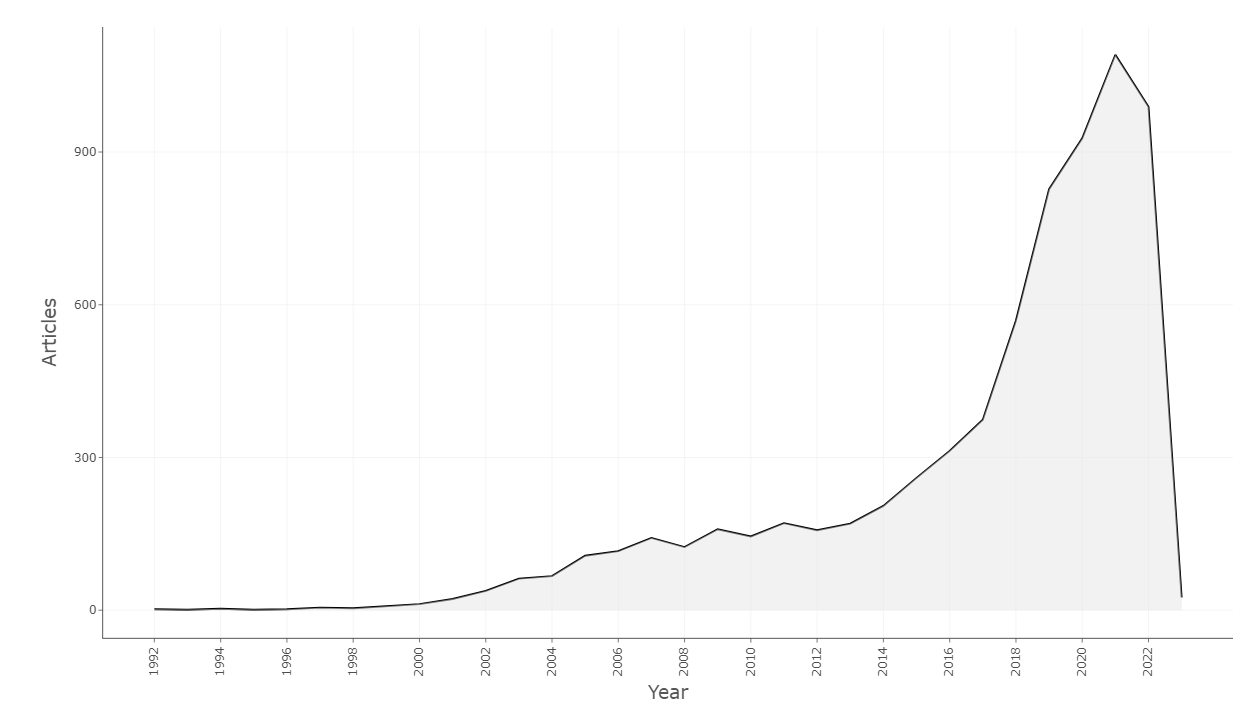
\includegraphics[scale=0.3]{images/evolucaoclassificacao.png}
    \label{fig:historicotexto}
    \end{center}
     \small\textbf{Origem:}  O autor.
\end{figure}

\section{Principais Jornais e Conferências}

Com relação a jornais e conferências, a Tabela \ref{tab:origem-acumulado} mostra que não há uma concentração significativa de publicações. As dez principais fontes representam 12,2\% do total de publicações, o que demonstra uma ampla aplicabilidade do tema. É importante mencionar o primeiro jornal, que é um periódico de acesso aberto na Europa. Os próximos dois são repositórios tradicionais de artigos científicos nas áreas: ACM e IEEE. Outro jornal a se destacar é "Expert Systems With Applications". Além disso, vale mencionar que existem mais de 3600 fontes e mais de 14.000 autores envolvidos na amostra coletada.

\begin{table}[h]
\centering
\begin{tabular}{ >{\raggedright\arraybackslash}m{5cm} | >{\raggedleft\arraybackslash}m{1.5cm} | >{\raggedleft\arraybackslash}m{1.5cm} | >{\raggedleft\arraybackslash}m{1.5cm} }
\hline
\textbf{Origem} & \textbf{Quant.} & \textbf{Total} & \textbf{\%} \\ \hline
\makecell[{{p{5cm}}}]{CEUR Workshop Proceedings} & 228 & 228 & 3,2 \\ \hline
\makecell[{{p{5cm}}}]{ACM International Conference Proceeding Series} & 143 & 371 & 5,2 \\ \hline
IEEE Access & 133 & 504 & 7,0 \\ \hline
\makecell[{{p{5cm}}}]{Expert Systems with Applications} & 68 & 572 & 8,0 \\ \hline
Journal of Biomedical Informatics & 60 & 632 & 8,8 \\ \hline
Applied Sciences-Basel & 52 & 684 & 9,5 \\ \hline
\makecell[{{p{5cm}}}]{Journal of Physics: Conference Series} & 52 & 736 & 10,3 \\ \hline
Neurocomputing & 49 & 785 & 10,9 \\ \hline
\makecell[{{p{5cm}}}]{IJCAI International Joint Conference on Artificial Intelligence} & 48 & 833 & 11,6 \\ \hline
\makecell[{{p{5cm}}}]{International Journal of Advanced Computer Science and Applications} & 41 & 874 & 12,2 \\ \hline
\end{tabular}
\caption{Principais fontes de publicações sobre classificação de textos, quantidade de artigos por fonte, total acumulado e porcentagem do total de publicações.}
\label{tab:origem-acumulado}
\end{table}

\section{Artigos Mais Citados}

A Tabela \ref{tab:autores-titulos} apresenta uma lista de artigos de referência na área de classificação de texto, ordenados por número de citações. Destacam-se os trabalhos que tratam de técnicas de pré-processamento e modelos de aprendizado de máquina relevantes para a classificação de descrições de produtos, como técnicas para evitar super ajuste do aprendizado \cite{srivastava2014dropout}, aprendizado de transferência \cite{pan2010survey}, e métricas de desempenho \cite{sokolova2009systematic}.

\begin{table}[h]
\centering
\begin{tabular}{ >{\raggedright\arraybackslash}m{8cm} | >{\raggedleft\arraybackslash}m{2.5cm} | >{\raggedleft\arraybackslash}m{1.5cm} }
\hline
\textbf{Título} & \textbf{Citações} & \textbf{Ano} \\ \hline
\cite{srivastava2014dropout} & 19002 & 2014 \\ \hline
\cite{pan2010transfer} & 9633 & 2010 \\ \hline
\cite{sebastiani2002machine} & 3854 & 2002 \\ \hline
\cite{sokolova2009systematic} & 2472 & 2009 \\ \hline
\cite{zhang2007mlknn} & 1852 & 2007 \\ \hline
\cite{forman2003extensive} & 1843 & 2003 \\ \hline
\cite{le2014distributed} & 1772 & 2014 \\ \hline
\cite{quoc2014distributed} & 1663 & 2014 \\ \hline
\cite{dave2003mining} & 1483 & 2003 \\ \hline
\cite{tong2002support} & 1445 & 2002 \\ \hline
\cite{joachims2006training} & 1417 & 2006 \\ \hline
\cite{lai2015recurrent} & 1251 & 2015 \\ \hline
\cite{kusner2015word} & 1133 & 2015 \\ \hline
\cite{howard2018universal} & 1116 & 2018 \\ \hline
\cite{raffel2020exploring} & 1056 & 2020 \\ \hline
\cite{raina2007self} & 998 & 2007 \\ \hline
\cite{bottou2018optimization} & 876 & 2018 \\ \hline
\cite{tschantaridis2004support} & 841 & 2004 \\ \hline
\cite{natekin2013gradient} & 821 & 2013 \\ \hline
\cite{rennie2003tackling} & 760 & 2003 \\ \hline
\end{tabular}
\caption{Artigos mais citados na área de classificação de textos, incluindo número de citações e ano de publicação.}
\label{tab:autores-titulos}
\end{table}

\section{Discussão}

A classificação de textos curtos concentra-se em textos com até 200 caracteres, sendo comum em aplicações como análise de sentimentos em redes sociais e classificação de opiniões em resenhas de produtos. Devido ao comprimento limitado, técnicas de pré-processamento e extração de características são fundamentais para capturar as informações mais relevantes.

Devido ao comprimento limitado dos textos, as técnicas de classificação de texto curto geralmente se concentram em capturar as características mais relevantes dos textos para a classificação. Isso pode incluir técnicas de pré-processamento para remover stop words e normalizar o texto, bem como técnicas de extração de características para resumir o conteúdo do texto em um conjunto de características relevantes.

Além disso, a classificação de texto curto também pode se beneficiar de técnicas de aprendizado de máquina, como redes neurais, que podem ser treinadas para capturar padrões complexos nos textos curtos. Embora os modelos de linguagem como word2VEC e BERT sejam muito populares para classificação de texto mais longo, também existem modelos de linguagem específicos para classificação de texto curto, como ULMFiT, que foram projetados para lidar com textos curtos.

Em geral, a classificação de texto curto é uma área em constante evolução, e os 153 artigos encontrados demonstram a crescente importância dessa área. A combinação de técnicas de pré-processamento, extração de características e aprendizado de máquina tem permitido o desenvolvimento de modelos cada vez mais precisos e eficientes para classificar textos curtos.

\section{Lacunas na Literatura}

Apesar do avanço significativo nas técnicas de classificação de textos, algumas lacunas foram identificadas na literatura. Há uma carência de estudos focados especificamente na classificação de textos curtos em português, bem como uma falta de comparações sistemáticas entre diferentes abordagens de pré-processamento e algoritmos de classificação. Além disso, poucos estudos exploram o impacto das variações regionais do idioma português na eficácia dos modelos de classificação.

\section{Análise Crítica}

A análise dos estudos revisados revela que as técnicas de aprendizado de máquina, como SVM, Naive Bayes e redes neurais, são amplamente utilizadas para a classificação de textos curtos. No entanto, a eficácia dessas técnicas varia significativamente dependendo das estratégias de pré-processamento adotadas. Estudos que utilizam técnicas avançadas de pré-processamento, como lematização e remoção de stopwords, tendem a apresentar melhores resultados de acurácia e F1-score. Por outro lado, alguns estudos apontam desafios relacionados à sobreajuste e a necessidade de otimização dos hiperparâmetros para cada modelo. A aplicação de modelos de linguagem, como word2VEC e BERT, tem mostrado resultados promissores, mas a adaptação desses modelos para o português ainda é um campo em desenvolvimento.

% \section{Limitações do Estudo}

% Esta revisão sistemática apresenta algumas limitações que devem ser consideradas ao interpretar os resultados. Primeiramente, a pesquisa foi limitada a artigos em inglês e português, o que pode ter excluído estudos relevantes publicados em outros idiomas. Além disso, apenas artigos de jornais e conferências foram incluídos, excluindo teses, dissertações e literatura cinzenta que poderiam conter informações valiosas. Outra limitação é a potencial variabilidade na qualidade dos estudos incluídos, que pode influenciar os resultados e conclusões da revisão. Finalmente, a rápida evolução das técnicas de classificação de textos pode significar que alguns estudos recentes não foram capturados devido ao tempo necessário para a publicação e indexação dos artigos.


% \chapter{Revisão Sistemática}

% \section{Introdução}

% \section{Introdução}

% Esta revisão sistemática tem como objetivo identificar e analisar os estudos mais relevantes sobre técnicas de classificação de textos curtos, com um foco particular em descrições de produtos em português. 


% \section{Métodos}

% A pesquisa de literatura foi conduzida nas bases Scopus e Web of Science, utilizando os seguintes termos de pesquisa: "text* classification*" OR "text* categori\$ation*" OR "document* classification*" OR "document* categori\$ation*" e "machine learning" OR "machine* learn*" OR "ML" OR "artificial intelligence" OR "AI". A busca foi limitada aos idiomas Inglês e Português, abrangendo títulos, resumos e palavras-chave. Apenas artigos de jornais e conferências foram incluídos. Os critérios de inclusão foram: relevância para a classificação de textos curtos, enfoque em técnicas de aprendizado de máquina ou recuperação da informação, e pertinência ao contexto do idioma português. Artigos duplicados, revisões, e publicações sem acesso ao texto completo foram excluídos.


% % Apresenta-se uma pesquisa de literatura sobre as bases Scopus e Web of Science, utilizando-se os termos de pesquisa ( "text* classification*"  OR  "text* categori\$ation*"  OR  "document* classification*"  OR  "document* categori\$ation*" ) como primeiro tema e ("machine learning" OR "machine* learn*" OR "ML" OR "artificial intelligence" OR "AI") como segundo tema.  Foram limitados para o idioma Inglês e Português, busca no título, abstract e palavras chaves e limitando apenas a jornais e conferências.

% \section{Evolução das Palavras Chaves}

% As análises destacadas são evolução das palavras chaves, principais jornais e conferências da área, artigos mais citados e evolução da quantidade de publicações no tempo.

% A quantidade de artigos encontrados foi de 7169, tendo o assunto de classificação de texto um crescimento de 8,49\% ao ano.  A Figura \ref{fig:historicotexto} apresenta um pico em 2021 e um leve decrescimento para 2021, mas já apresentando artigos para o tema para o ano de 2023.  Verifica-se um rápido crescimento nos últimos anos no tema, isto é justificado pelo fato da tarefa estar diretamente aplicada a função de organização da informação.  

% \begin{figure}[htb]
%     \caption{Evolução Histórica dos artigos sobre classificação de texto nos últimos anos}
%     \begin{center}    
%     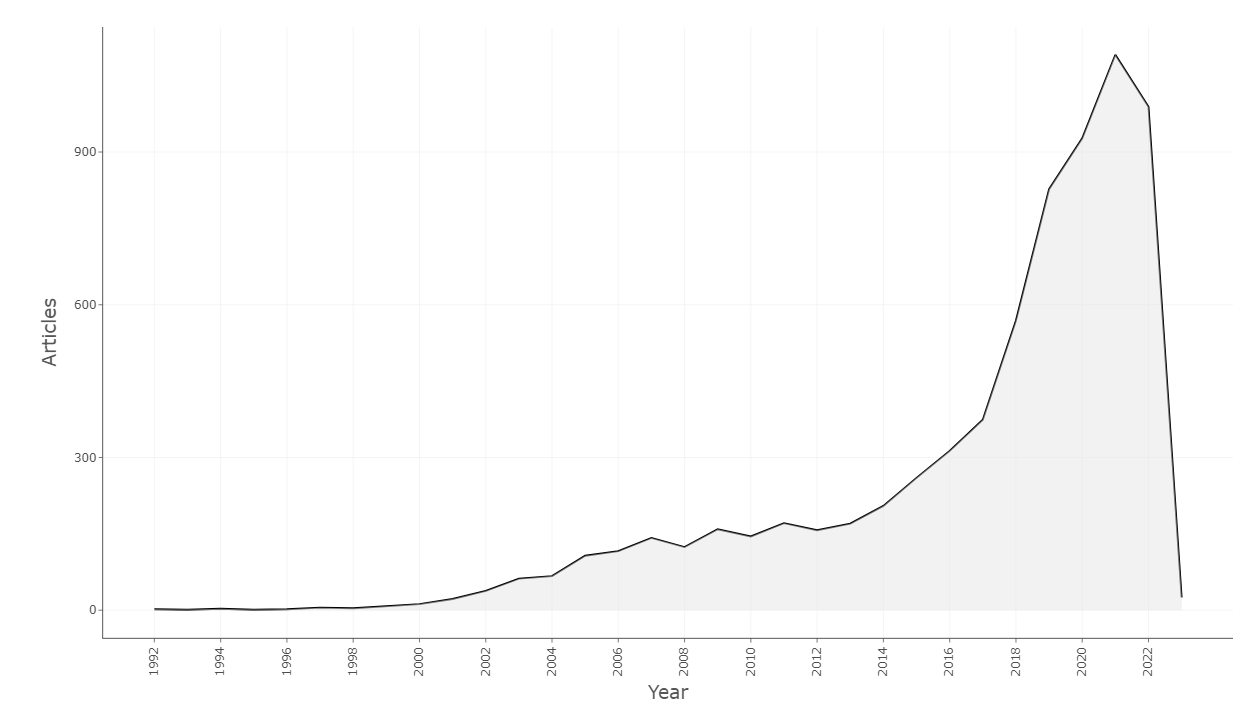
\includegraphics[scale=0.3]{images/evolucaoclassificacao.png}
%     \label{fig:historicotexto}
%     \end{center}
%      \small\textbf{Origem:}  O autor.
% \end{figure}

% \section{Principais Jornais e Conferências}

% Com relação a jornais e conferências, a Tabela \ref{tab:origem-acumulado} mostra que não há uma concentração significativa de publicações. As dez principais fontes representam 12,2\% do total de publicações, o que demonstra uma ampla aplicabilidade do tema. É importante mencionar o primeiro jornal, que é um periódico de acesso aberto na Europa. Os próximos dois são repositórios tradicionais de artigos científicos nas áreas: ACM e IEEE. Outro jornal a se destacar é "Expert Systems With Applications". Além disso, vale mencionar que existem mais de 3600 fontes e mais de 14.000 autores envolvidos na amostra coletada.


% \begin{table}[h]
% \centering
% \begin{tabular}{ >{\raggedright\arraybackslash}m{5cm} | >{\raggedleft\arraybackslash}m{1.5cm} | >{\raggedleft\arraybackslash}m{1.5cm} | >{\raggedleft\arraybackslash}m{1.5cm} }
% \hline
% \textbf{Origem} & \textbf{Quant.} & \textbf{Total} & \textbf{\%} \\ \hline
% \makecell[{{p{5cm}}}]{CEUR Workshop Proceedings} & 228 & 228 & 3,2 \\ \hline
% \makecell[{{p{5cm}}}]{ACM International Conference Proceeding Series} & 143 & 371 & 5,2 \\ \hline
% IEEE Access & 133 & 504 & 7,0 \\ \hline
% \makecell[{{p{5cm}}}]{Expert Systems with Applications} & 68 & 572 & 8,0 \\ \hline
% Journal of Biomedical Informatics & 60 & 632 & 8,8 \\ \hline
% Applied Sciences-Basel & 52 & 684 & 9,5 \\ \hline
% \makecell[{{p{5cm}}}]{Journal of Physics: Conference Series} & 52 & 736 & 10,3 \\ \hline
% Neurocomputing & 49 & 785 & 10,9 \\ \hline
% \makecell[{{p{5cm}}}]{IJCAI International Joint Conference on Artificial Intelligence} & 48 & 833 & 11,6 \\ \hline
% \makecell[{{p{5cm}}}]{International Journal of Advanced Computer Science and Applications} & 41 & 874 & 12,2 \\ \hline
% \end{tabular}
% \caption{Principais fontes de publicações sobre classificação de textos, quantidade de artigos por fonte, total acumulado e porcentagem do total de publicações.}
% \label{tab:origem-acumulado}
% \end{table}



% % A Tabela \ref{tab:autores-titulos} apresenta uma lista de artigos de referência na área de aprendizado de máquina para classificação de texto, ordenados por número de citações. É possível observar que os artigos mais citados tratam de técnicas para evitar super ajuste do aprendizado e como o método "Dropout" proposto pode auxiliar \cite{srivastava2014dropout}, bem como estudos sobre aprendizado de transferência \cite{pan2010survey} e métricas de desempenho para tarefas de classificação \cite{sokolova2009systematic}. Outros tópicos abordados incluem aprendizado passivo \cite{zhang2007mlknn}, seleção de recursos \cite{forman2003extensive}, representações distribuídas de sentenças e documentos \cite{le2014distributed} e modelos de processamento de linguagem natural como o "Universal Language Model Finetuning" \cite{howard2018universal}.
% % É importante notar que esses artigos abrangem muitos anos de publicação, desde 2002 até 2020, e isso demonstra que a área tem-se desenvolvido constantemente e continuará a desenvolver-se no futuro.

% \section{Artigos Mais Citados}

% A Tabela \ref{tab:autores-titulos} apresenta uma lista de artigos de referência na área de classificação de texto, ordenados por número de citações. Destacam-se os trabalhos que tratam de técnicas de pré-processamento e modelos de aprendizado de máquina relevantes para a classificação de descrições de produtos, como técnicas para evitar super ajuste do aprendizado \cite{srivastava2014dropout}, aprendizado de transferência \cite{pan2010survey}, e métricas de desempenho \cite{sokolova2009systematic}.


% \usepackage{makecell}
% \usepackage{array}

% \begin{table}[h]
% \centering
% \begin{tabular}{ >{\raggedright\arraybackslash}m{8cm} | >{\raggedleft\arraybackslash}m{2.5cm} | >{\raggedleft\arraybackslash}m{1.5cm} }
% \hline
% \textbf{Título} & \textbf{Citações} & \textbf{Ano} \\ \hline
% \cite{srivastava2014dropout} & 19002 & 2014 \\ \hline
% \cite{pan2010transfer} & 9633 & 2010 \\ \hline
% \cite{sebastiani2002machine} & 3854 & 2002 \\ \hline
% \cite{sokolova2009systematic} & 2472 & 2009 \\ \hline
% \cite{zhang2007mlknn} & 1852 & 2007 \\ \hline
% \cite{forman2003extensive} & 1843 & 2003 \\ \hline
% \cite{le2014distributed} & 1772 & 2014 \\ \hline
% \cite{quoc2014distributed} & 1663 & 2014 \\ \hline
% \cite{dave2003mining} & 1483 & 2003 \\ \hline
% \cite{tong2002support} & 1445 & 2002 \\ \hline
% \cite{joachims2006training} & 1417 & 2006 \\ \hline
% \cite{lai2015recurrent} & 1251 & 2015 \\ \hline
% \cite{kusner2015word} & 1133 & 2015 \\ \hline
% \cite{howard2018universal} & 1116 & 2018 \\ \hline
% \cite{raffel2020exploring} & 1056 & 2020 \\ \hline
% \cite{raina2007self} & 998 & 2007 \\ \hline
% \cite{bottou2018optimization} & 876 & 2018 \\ \hline
% \cite{tschantaridis2004support} & 841 & 2004 \\ \hline
% \cite{natekin2013gradient} & 821 & 2013 \\ \hline
% \cite{rennie2003tackling} & 760 & 2003 \\ \hline
% \end{tabular}
% \caption{Artigos mais citados na área de classificação de textos, incluindo número de citações e ano de publicação.}
% \label{tab:autores-titulos}
% \end{table}


% A classificação de texto é um tema que tem evoluído ao longo dos anos, e que pode ser dividido em três eixos: preparação da informação, técnicas e aplicações. No que diz respeito à preparação da informação, a evolução do tema começou com técnicas determinísticas, seguidas por técnicas estatísticas e matriciais. Mais recentemente, a aplicação de redes neurais tem permitido o desenvolvimento de modelos de linguagem aprimorados, como word2VEC e BERT.

% No eixo das técnicas, a tendência foi semelhante, iniciando-se com técnicas determinísticas, seguida por técnicas matriciais. No entanto, houve uma grande aplicação de técnicas de aprendizado de máquina, como KNN, Naive Bayes e SVM, seguida por técnicas agregadas, como Ensemble e Boosting. Mais recentemente, tem-se utilizado diversas arquiteturas de redes neurais, como CNN, RNN, modelos de Atenção e Transformers.

% Por fim, no eixo das aplicações, é possível ver a versatilidade da área de classificação de texto. As aplicações estão presentes em campos como a saúde, o direito, a identificação de autoria, a exploração de sentimentos em redes sociais e linguagens específicas, como Chinês e Árabe. Além disso, aplicações como chatbot, sumarização de texto, classificação hierárquica e bulling também são mencionadas. A lista de aplicações levantadas inclui mais de 50 exemplos.

% Em resumo, a classificação de texto é um tema amplo e em constante evolução, que abrange desde a preparação da informação até as técnicas e aplicações mais recentes. A utilização de técnicas estatísticas e matriciais, seguida pela utilização de redes neurais, tem permitido o desenvolvimento de modelos cada vez mais precisos e eficientes. Além disso, as aplicações são amplas e abrangem diferentes campos e linguagens.




% \section{Discussão}

% A classificação de textos curtos concentra-se em textos com até 200 caracteres, sendo comum em aplicações como análise de sentimentos em redes sociais e classificação de opiniões em resenhas de produtos. Devido ao comprimento limitado, técnicas de pré-processamento e extração de características são fundamentais para capturar as informações mais relevantes.

% Devido ao comprimento limitado dos textos, as técnicas de classificação de texto curto geralmente se concentram em capturar as características mais relevantes dos textos para a classificação. Isso pode incluir técnicas de pré-processamento para remover stop words e normalizar o texto, bem como técnicas de extração de características para resumir o conteúdo do texto em um conjunto de características relevantes.

% Além disso, a classificação de texto curto também pode se beneficiar de técnicas de aprendizado de máquina, como redes neurais, que podem ser treinadas para capturar padrões complexos nos textos curtos. Embora os modelos de linguagem como word2VEC e BERT sejam muito populares para classificação de texto mais longo, também existem modelos de linguagem específicos para classificação de texto curto, como ULMFiT, que foram projetados para lidar com textos curtos.

% Em geral, a classificação de texto curto é uma área em constante evolução, e os 153 artigos encontrados demonstram a crescente importância dessa área. A combinação de técnicas de pré-processamento, extração de características e aprendizado de máquina tem permitido o desenvolvimento de modelos cada vez mais precisos e eficientes para classificar textos curtos.

% \section{Lacunas na Literatura}

% Apesar do avanço significativo nas técnicas de classificação de textos, algumas lacunas foram identificadas na literatura. Há uma carência de estudos focados especificamente na classificação de textos curtos em português, bem como uma falta de comparações sistemáticas entre diferentes abordagens de pré-processamento e algoritmos de classificação. Além disso, poucos estudos exploram o impacto das variações regionais do idioma português na eficácia dos modelos de classificação.

% \section{Análise Crítica}

% A análise dos estudos revisados revela que as técnicas de aprendizado de máquina, como SVM, Naive Bayes e redes neurais, são amplamente utilizadas para a classificação de textos curtos. No entanto, a eficácia dessas técnicas varia significativamente dependendo das estratégias de pré-processamento adotadas. Estudos que utilizam técnicas avançadas de pré-processamento, como lematização e remoção de stopwords, tendem a apresentar melhores resultados de acurácia e F1-score. Por outro lado, alguns estudos apontam desafios relacionados à sobreajuste e a necessidade de otimização dos hiperparâmetros para cada modelo. A aplicação de modelos de linguagem, como word2VEC e BERT, tem mostrado resultados promissores, mas a adaptação desses modelos para o português ainda é um campo em desenvolvimento.


% \section{Análise Crítica}

% A classificação de textos curtos concentra-se em textos com até 200 caracteres, sendo comum em aplicações como análise de sentimentos em redes sociais e classificação de opiniões em resenhas de produtos. Devido ao comprimento limitado, técnicas de pré-processamento e extração de características são fundamentais para capturar as informações mais relevantes.



% % Classificação de texto curto é uma área específica da classificação de texto que se concentra em classificar textos com comprimentos curtos, geralmente até 200 caracteres. Esta área é comumente utilizada em aplicações como análise de sentimento em redes sociais, onde os comentários e postagens são curtos, e classificação de opiniões em resenhas de produtos, entre outras.

% Devido ao comprimento limitado dos textos, as técnicas de classificação de texto curto geralmente se concentram em capturar as características mais relevantes dos textos para a classificação. Isso pode incluir técnicas de pré-processamento para remover stop words e normalizar o texto, bem como técnicas de extração de características para resumir o conteúdo do texto em um conjunto de características relevantes.

% Além disso, a classificação de texto curto também pode se beneficiar de técnicas de aprendizado de máquina, como redes neurais, que podem ser treinadas para capturar padrões complexos nos textos curtos. Embora os modelos de linguagem como word2VEC e BERT sejam muito populares para classificação de texto mais longo, também existem modelos de linguagem específicos para classificação de texto curto, como ULMFiT, que foram projetados para lidar com textos curtos.

% Em geral, classificação de texto curto é uma área em constante evolução, e os 153 artigos encontrados demonstram a crescente importância dessa área. A combinação de técnicas de pré-processamento, extração de características e aprendizado de máquina tem permitido o desenvolvimento de modelos cada vez mais precisos e eficientes para classificar textos curtos.
